% Author: Izaak Neutelings (June, 2018)
\documentclass[border=3pt,tikz]{standalone}
\usepackage{ifthen}
\usepackage{siunitx}
\usepackage{tikz}
\usetikzlibrary{hobby} % for ..
\usetikzlibrary{arrows.meta} % to control arrow size
\tikzset{>={Latex[length=4,width=4]}} % for LaTeX arrow head
\usetikzlibrary{calc,intersections,decorations.markings}
\usepackage{siunitx}
\usepackage{xcolor} % for colored text

\colorlet{mylightblue}{blue!20}
\colorlet{myblue}{blue!50!black}
\colorlet{mydarkblue}{blue!30!black}
\colorlet{mylightred}{red!10}
\colorlet{myred}{red!50!black}
\colorlet{mydarkred}{red!60!black}
\colorlet{mydarkgreen}{green!30!black}

%\tikzstyle{midarr}=[decoration={markings,mark=at position 0.5 with {\arrow{stealth}}},postaction={decorate}]
\tikzset{
    midarr/.style={decoration={markings,mark=at position #1 with {\arrow{stealth}}},postaction={decorate}},
    midarr/.default=0.5
}
\def\tick#1#2{\draw[thick] (#1) ++ (#2:0.03*\ymax) --++ (#2-180:0.06*\ymax)}


\begin{document}


% PHASE TRANSITIONS
    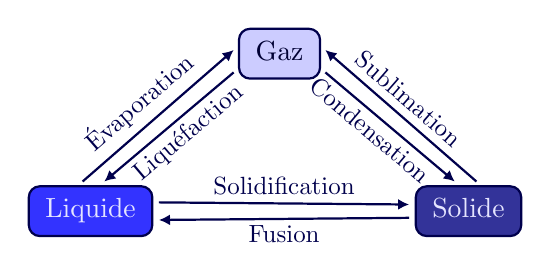
\begin{tikzpicture}[arrow/.style={->,thick,mydarkblue,shorten <=2,shorten >=2},
    box/.style={thick,rounded corners=4,inner xsep=6,inner ysep=3}]
    \message{Phase transitions^^J}

    \node[blue!10!white,draw=mydarkblue,fill=blue!80!white,box] (S) at (-2.4,0) {\strut Liquide};
    \node[blue!10!white,draw=mydarkblue,fill=blue!50!gray!80!black,box] (L) at (2.4,0) {\strut Solide};
    \node[blue!20!black,draw=mydarkblue,fill=blue!20!white,box] (G) at (0,2) {\strut Gaz};

    \draw[arrow,->] (S.8) -- (L.173) node[above,midway,scale=0.9] {Solidification};
    \draw[arrow,->] (L.-173) -- (S.-8) node[below=-1pt,midway,scale=0.9] {Fusion};

    \draw[arrow,->] (S.115) -- (G.-190) node[left=2pt,above,midway,sloped,scale=0.9] {Évaporation};
    \draw[arrow,->] (G.-160) -- (S.70) node[left=-4pt,below=-1pt,midway,sloped,scale=0.9] {Liquéfaction};

    \draw[arrow,->] (L.65) -- (G.10) node[left=2pt,above,midway,sloped,scale=0.9] {Sublimation};
    \draw[arrow,->] (G.-20) -- (L.110) node[left=5pt,below=-1pt,midway,sloped,scale=0.9] {Condensation};

    \end{tikzpicture}

\end{document}
